\documentclass[a4paper]{scrreprt}
\usepackage{fancyhdr}
\pagestyle{fancy}
\usepackage[english]{babel}
\usepackage[utf8]{inputenc}

\usepackage{graphicx}
\usepackage{url}
\usepackage{textcomp}
\usepackage{amsmath}
\usepackage{lastpage}
\usepackage{pgf}
\usepackage{wrapfig}
\usepackage{fancyvrb}
\usepackage{float}

%\usepackage[style=ieee]{biblatex} % om du vill köra ieee (tror leif kör den)
\usepackage[backend=biber,style=vancouver]{biblatex}
\addbibresource{bibfile.bib}
%Alternativt med natbib
%\usepackage[numbers]{natbib} %referenser vancouver
%\usepackage[numbers,round]{natbib} %referenser vancouver
%\usepackage{hyperref}

\usepackage{pdflscape}
% \usepackage{lscape}

% Code highligting
% \usepackage{minted}
\usepackage[outputdir=output/tex]{minted} % iom min makefile



\usepackage[font=footnotesize,labelfont=bf,skip=2pt]{caption}
\usepackage{hyperref}
\newenvironment{longlisting}{\captionsetup{type=listing}}{}
% \renewcommand\listoflistingscaption{Källkod....}
\renewcommand\listoflistingscaption{List of source codes}
\setmintedinline[java]{breaklines=true,breakanywhere=true} % necessary for breakanywhere to work later on.

\usepackage{paralist} %Inline lists

% Create header and footer
\headheight 27pt
\pagestyle{fancyplain}
\lhead{\footnotesize{Object-Oriented Design, IV1350}}
\chead{}
\rhead{\footnotesize{Seminar 4 Additional Higher Grade Tasks}}
\lfoot{}
\cfoot{\thepage\ (\pageref{LastPage})}
\rfoot{}

% Create title page
\title{Additional Higher Grade Tasks}
\subtitle{Object-Oriented Design, IV1350}
\author{Vincent Ferrigan ferrigan@kth.se}

\begin{document}

\maketitle

\tableofcontents %Generates the TOC

\chapter{Introduction}
The purpose of this report is to
add to the higher grade score.

% TODO: Explain in short which tasks you have chosen to pursue and what you have been instructed to do.

\chapter{Method}
\section*{Tools}
This project was implemented in \emph{Java}.
The UML modeling tool used was \emph{PlantUML}.
PlantUML is an open-source tool for creating UML diagrams using a text-based
syntax.
It was chosen to enable version control through git and to avoid using a
proprietary graphical editor.
This report was also written in plain text mode -- \LaTeX.

All code was written in \emph{IntelliJ IDEA} and the unit tests were written with the \emph{JUnit 5} test framework.
Quick-fixes and editing was, however, done in \emph{Vim}.

\section*{The project's resources and the system's configuration and data}
\label{sec:resources}
Instead of hard-coding data in the integration classes,
flat file databases are used to store records.
These CSV-files store,
read and update data for accounting, inventory (a product catalog included), and customer details.

The filenames and their paths are all found in the project's \verb|Config.Properties|
file under \verb|src/main/resources|.
The class names of the objects a \emph{Factory} can create, and the filenames of all the loggers are also
configured in the same file.

The properties are added to the \verb|System Properties| -- a set-up based on
\href{https://docs.oracle.com/javase/tutorial/essential/environment/sysprop.html}{The Java\texttrademark{} Tutorials - System Properties}

If a developer is having trouble loading the resource file \verb|config.properties|,
they will have to first check that the \verb|src/main/resources|
is correctly configured as a resource directory in your IDE.

Since the system reads and writes to files, handling exceptions became necessary.

\section*{Tests}
Tests are created using the JUnit 5 framework and follow best practice, i.e., they
have the same directory architecture as the program, and are placed outside the source
folder for the program (the SUT).

Similar to the SUT, the tests have their own Config Properties file, error-log file and flat file databases
(see listing ~\ref{listing:test-config.properties}) and are added to the \verb|System Properties| with
a \mintinline{java}{@BeforeAll} method (see listing ~\ref{listing:before-all-tests-setup}).

In this way, the inventory can be changed on the fly, just by manipulating
the \verb|inventory_items.csv| file which is placed \verb|test-data/db| directory.
The test can create, compare and manipulate its own database and log-files.
This enables testing classes in both the integration and util layer package.
. %TYP TODO men har du gjort så? Lägg till ErrorFileLogHandler test, TotalRevenueFileOutput test.

\begin{longlisting}
    \inputminted[
        label=@BeforeAll tests setup,
        linenos=true,
        bgcolor=lightgray,
        firstline=1,
        lastline=25,
%        frame=single,
        fontsize=\footnotesize,
    ]{bash}{../../src/test/resources/config.properties}
    \caption{The Config Properties file for the JUnit tests.}
    \label{listing:test-config.properties}
\end{longlisting}

\newpage
\begin{longlisting}
    \inputminted[
        label=@BeforeAll tests setup,
        linenos=true,
        bgcolor=lightgray,
        firstline=10,
        lastline=34,
%        frame=single,
        fontsize=\footnotesize,
    ]{java}{../../src/test/se/kth/iv1350/POSTestSuperClass.java}
    \caption{The Config Properties are added to the System Properties in a @BeforeAll setup method.
    This method is placed in a superclass, which is extended in all test that require a pre-configruation}
    \label{listing:before-all-tests-setup}
\end{longlisting}

\section*{The overall Work-flow}
\section*{Task 1, Inheritance}
\section*{Task 2, Inheritance vs Composition}
\section*{Task 3, Testing Output}

\newpage
\chapter{Result}
\label{sec:result}
The entire program, including the additional tasks can be found here on GitHub:

\subsubsection*{GitHub-Repo}
\url{https://github.com/VincentFerrigan/kth-iv1350-object-oriented-design}

\section*{Task 1, Inheritance}
Since the observers perform similar steps in the same order,
the Template Method design-pattern can be applied.
In this way duplicated code can be eliminated.

\begin{figure}[H]
    \begin{center}
        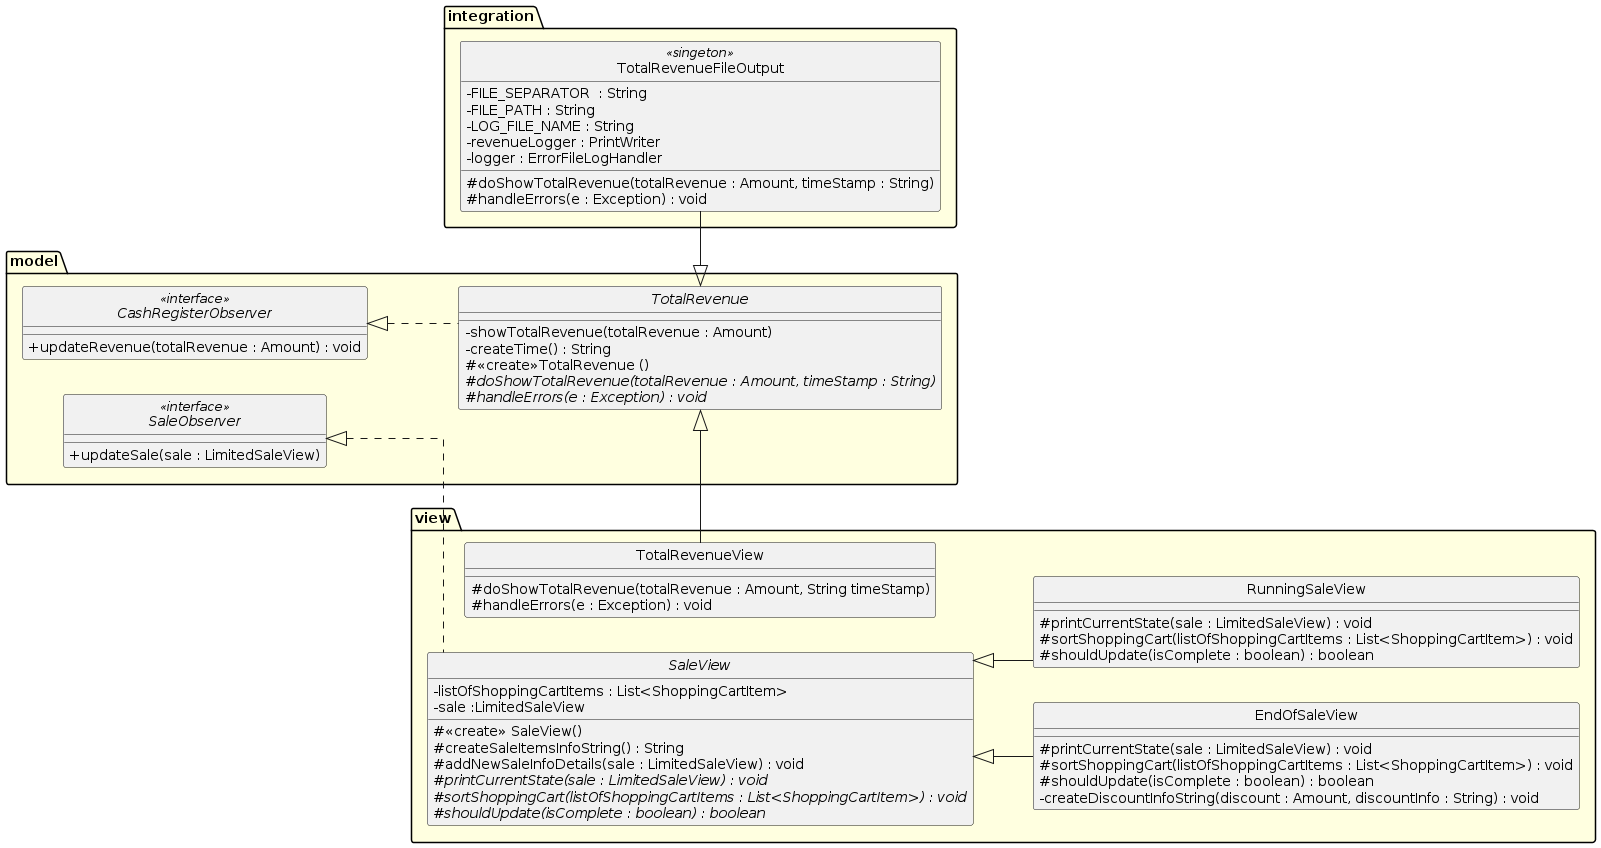
\includegraphics[width=\textwidth]{../../uml/output/uml_adp_tasks}
%        \includegraphics[trim=0cm 0cm 0cm 0cm, clip, width=\textwidth]{uml/output/uml_v3.png}
%        \caption{The Start Up \verb|Main| system operations}
        \caption{The template method applied with the observer pattern.
        This UML is an extract from the main class diagram.\\}
        \label{fig:the-observers}
    \end{center}
\end{figure}

The abstract class
\mintinline{java}{SaleView} is the template
for sale observers\footnote{The observers are only exposed to certain methods or attributes.
For example, a limited view of a particular sale is sent to the
sale observers by using an ''observered-interface'' called
\mintinline{java}{LimitedSaleView}.
This interface is implemented by the wrapper class
\mintinline{java}{LimitedSaleViewWrapper} that
only exposes certain Sale methods.}
\mintinline{java}{RunningSaleView} and
\mintinline{java}{EndOfSaleView},
while the abstract class
\mintinline{java}{TotalRevenue}
acts as the template for cash register observers
\mintinline{java}{TotalRevenueView} and
\mintinline{java}{TotalRevenueFileOutput}.
The class diagram for the observer and template method pattern
is illustrated in figure ~\ref{fig:the-observers}.

As mentioned above, the template method
is not only applied on the task at hand (revenue updates),
but also for the observers that display sale details.
The display of sale details is updated each time an item is added to the shopping cart
and during end-of-sale performed in order to display possible discounts.
The display of the total revenue, including revenue logging to a file, is updated
each time a sale is paid for.
The outcome of refactoring to both the observer-pattern and template method
is demonstrated in all samples that are included in the README file,
and therefore presented on the GitHub repository page.

\section*{Task 2, Inheritance vs Composition}
\section*{Task 3, Testing Output}

%\begin{longlisting}
%    \inputminted[
%        label=The common Discount-Strategy Interface,
%        linenos=true,
%        bgcolor=lightgray,
%        firstline=11,
%        lastline=21,
%%        frame=single,
%        fontsize=\footnotesize,
%    ]{java}{../../src/main/se/kth/iv1350/integration/pricing/DiscountStrategy.java}
%    \caption{Discount strategy defining the ability to calculate total price.
%        This interface shall be implemented by a class providing a promotion or
%        discount algorithm.}
%    \label{listing:discount-strategy}
%\end{longlisting}

\chapter{Discussion}
\label{sec:discussion}
\section*{The Template Model}
\section*{Inheritance vs Composition}
\section*{Testing Output}

%\appendix
%\chapter{UML -- The Refined Design}
%\subsection*{System Operations}
%\subsubsection*{The Start up, Main System Operation}
%\begin{figure}[H]
%    \begin{center}
%        \includegraphics[width=\textwidth]{../../uml/output/uml_v3_004}
%%        \includegraphics[trim=0cm 0cm 0cm 0cm, clip, width=\textwidth]{uml/output/uml_v3.png}
%%        \caption{The Start Up \verb|Main| system operations}
%        \caption{The Main System operation}
%        \label{fig:start-up}
%    \end{center}
%\end{figure}
%

\listoflistings % Now typeset the list
\printbibliography
%med natbib
%\bibliographystyle{unsrtnat} % referenser vancouver
\end{document}
